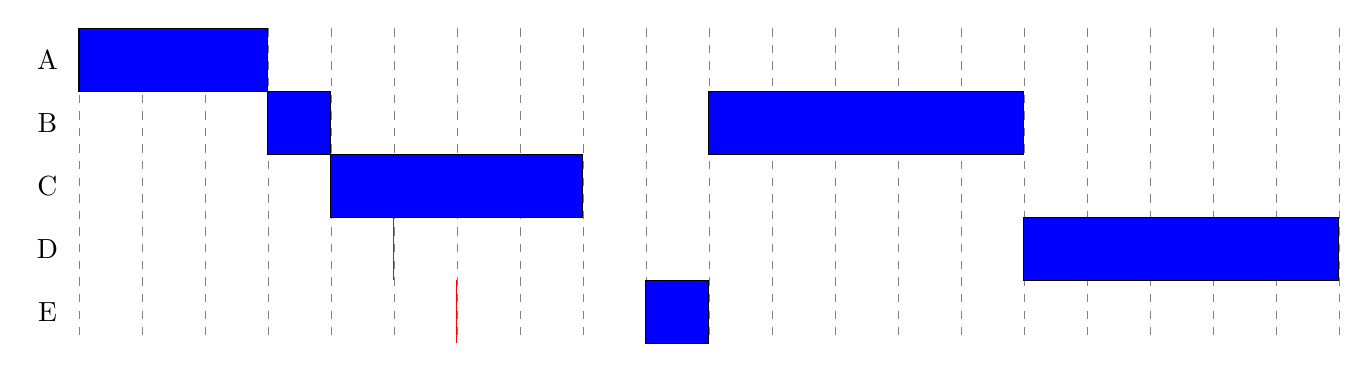
\begin{tikzpicture}[scale=.8]
   \foreach \i in {0,...,20}
   \draw[dashed, help lines] (\i,0) -- (\i,-5);

   \node (A) at (-.5,-.5) {A};
   \node (B) at (-.5,-1.5) {B};
   \node (C) at (-.5,-2.5) {C};
   \node (D) at (-.5,-3.5) {D};
   \node (E) at (-.5,-4.5) {E};

   \foreach \p in {0,...,4}
   \draw[red] (2+\p, -\p) --++ (0,-1);

   \draw[fill=blue] (0,0) rectangle (3,-1) rectangle (4,-2) rectangle (8,-3);
   \draw[fill=blue] (9,-5) rectangle (10,-4);
   \draw[fill=blue] (10,-2) rectangle (15,-1);
   \draw[fill=blue] (15,-3) rectangle (20,-4);

\end{tikzpicture}

% Tt     3  15     8    20    10    //
% Tr     3  13     4    14    2     7.2
% Tr/Ts  1  13/6   1    14/5  1     1.59